% Packages:
\begin{document}

\documentclass[12pt]{article}
\usepackage{graphicx}
\usepackage{booktabs}
\usepackage{listings}
\usepackage{xcolor}

\lstset{
  basicstyle=\ttfamily,
  frame=single,
  backgroundcolor=\color{lightgray!20},
  keywordstyle=\color{blue},
  commentstyle=\color{gray},
  stringstyle=\color{green},
  showstringspaces=false
}

\section{Title}
A Bayesian Network Model based decision support tool for Environmental Sustainability in the Australian Winegrowing Industry.

\section{Abstract}

Environmental sustainability in the Australian winegrowing industry involves complex, interacting factors. To address this, we developed a Bayesian Network (BN) model, integrating data and expert input to summarise key factors, their relationships, and impacts on vineyard outcomes. The BN model was iteratively refined, involving variable selection, structure definition, and probability estimation, with expert input ensuring industry relevance and regional adaptability. A case study of the Coonawarra region highlighted regional differences while underscoring industry-wide concerns, such as agrochemical use. The BN model, accessible via an application, allows for continuous industry feedback and adaptation. This study underscores the potential of BNs as powerful tools for sustainability analysis in agriculture, offering valuable insights for sustainable vineyard management.

\section{Introduction}

The imperative for environmental sustainability in agriculture has intensified as the sector strives to balance productivity with ecological preservation~\cite{baianoOverviewSustainabilityWine2021,corboEnvironmentalSustainabilityPrograms2014}. This is especially true for Viticulture, the cultivation of grapevines for wine production, as it presents unique challenges and opportunities for sustainability, particularly due to its position as a luxury good amongst other agricultural industries~\cite{longbottomExploringLinksSustainability2018,ferraraLifeCycleAssessment2018}. This study investigates environmental sustainability practices in Australian winegrowing, using the application of Bayesian Networks (BNs). To create a rigorous and quantitative approach to understanding sustainable practices and the relationships between factors associated with these practices, a broad model of Australian winegrowing was created. This model was followed by a more specific case study looking at the Coonawarra winegrowing region.

BNs are probabilistic models that capture and analyse the interactions between multiple factors in complex systems~\cite{korbBayesianArtificialIntelligence2011}. BNs also facilitate the integration of diverse types and sources of information, including expert knowledge, the results of prior experiements, outcomes from published literature, and so on. In this study, the BNs integrated expert knowledge and region-specific data within a structured framework to quantify the impacts of various factors on sustainability within Australian winegrowing. This methodology shed light on current sustainability practices, identified critical areas for intervention and facilitated evolution of the potential impact of various management action or climate scenarios.

This research is guided by several fundamental inquiries aimed at enhancing our understanding of environmental sustainability in viticulture. A primary question is how key factors impacting environmental sustainability can be rigorously defined and quantified. Another focus delves into identifying the unique regional characteristics of different regions, using the Coonawarra winegrowing region to illustrate how the relative influence of factors might change regionally. Additionally, the study investigates how these factors interact with each other. The final question is, how the findings from these Bayesian Network models compare with existing literature on sustainability in viticulture, aiming to connect industry perceptions to academic knowledge.

An industry panel comprising experts in viticulture and environmental sustainability, was convened to guide the project. The panel acted as a catalyst in the early stages of the research to help explore the above questions. The panel input was supported by a comprehensive literature review, which established a foundational understanding of the current knowledge landscape and identified major concepts within sustainable winegrowing. To ensure a robust and comprehensive BN, a combination of qualitative and quantitative methods were employed in its creation via expert consultations and data analysis. The study thus aimed to produce findings that are not only theoretically sound but also practically relevant and applicable to the viticulture industry.

\section{Methods}

In agriculture, the consideration of environment is critical to the success of the industry. The question of environmental sustainability has continued to grow in importance as the industry is affected by international market demands, disease pressures, natural disasters and social change \citep{wineaustraliaNationalVintageReport2022,wineaustraliaNationalVintageReport2020,wineaustraliaNationalVintageReport2021,cassonMultidisciplinaryApproachAssess2022}. The question of sustainability requires the consideration of a multitude of factors, not only due to physical characteristics and differences between locations and habitats but also due to priorities driven by diverse perspectives including consumers, produces, the community, government and industry \citep{baianoOverviewSustainabilityWine2021,wayeCarbonFootprintsFood2008}. It is important to consider each factor with respect to these perspectives, and to be explicit in how they are defined \citep{santiago-brownSustainabilityAssessmentWineGrape2015}.

Collaboration between experts from different perspectives helps to reconcile opinions regarding different factors and their contribution to sustainable outcomes \citep{dichiaraCollaborativeApproachAchieving2024}. In Australia, all of the above groups mentioned are  united in the priority to improve greenhouse gas emissions and resource inputs through approaches such as regulating chemicals, water use and fertilisers \citep{dumbrellComparingAustralianPublic2024}. While there is a general agreement on broader regulatory needs, the industry requirements vary greatly between different wine regions; due to climate, soil types and water resources \citep{abbalDecisionSupportSystem2016,agostaRegionalClimateVariability2012}.
% TODO:
% KM: I Suggest expanding this (the paragraph below) - split into measurement, methods, etc - or leave this para out and absorb refs into the lit review. G, K and F seem quite relevant but this paragraph doesnt do them justice so expand or move.
% 
% Review further comments about this paragraph - its not a good piece of work but it is important to consider how impact and sustainability is or could be measured and interpretted. Perhaps go deeper like you did in your confirmation.
Methods for measuring sustainability comprise a wide variety of approaches with the use of index systems being common \citep{gehringerMappingSustainabilityMeasurement2024}. Other approaches utilise the identification of key factors, and their measurements as a proxy to indicate impact to, or the health of, the environment \citep{floresWhatSustainabilityWine2018}. The measuring of sustainability through the use of these tools can help to manage risk and promote resilience for industries through identifying sustainable goals and key factors of interest that contribute to positive outcomes \citep{klemesAssessingMeasuringEnvironmental2015, beckerSustainabilityScienceManaging2024}. Within this study we focus on measuring key factors and establishing how they interact, and ultimately effect the surrounding environment; the chosen method for this study is a Bayesian Network.
%%%%%%%%%%%%%%%%%%%%%%%%%%%%%%%%%%%%%%%%%%%%%%%%%
% End suggestion.
%%%%%%%%%%%%%%%%%%%%%%%%%%%%%%%%%%%%%%%%%%%%%%%%%
\subsection{Literature Review}

The literature review was designed to access existing knowledge on environmental sustainability in viticulture with the aim of identifying key factors influencing sustainability and understanding their interactions.

These findings were combined with the information derived from the expert consultations to inform the BN construction and quantification. 
% Clarify that the review helped inform the strawman model and was only used as a comparison point afterwards.

A systematic search of terms, broadly based on key factors given from the industry panel, was conducted. The general query (adapted to different formats for various journals and bibliographic databases) used for the literature search was: 

% This is the query in a code-like format.
\begin{lstlisting}[language=]
    (Water OR Agrochemical OR Chemical OR Ground management OR Pest OR Disease OR Management OR Electricity OR Energy OR GHG OR Emissions OR Greenhouse gas emissions OR Environmental OR Environment OR Ecological OR Fertiliser OR Fertilizer OR Fuel OR Biofuel OR Price OR Nutrient OR Runoff OR Leeching OR Market OR Supply and demand OR Soil OR Organic carbon OR SOC OR Tractor OR Field OR Operations OR Weather OR Climate OR Yield OR Production)
    AND
    (Sustainability OR Sustainable OR Eco-friendly OR Environmentally friendly OR Green practices)
    AND
    (Viticulture OR Winegrowing OR Vineyard)
    \end{lstlisting}

Specific inclusion and exclusion criteria were applied in the literature search. Articles were only excluded if they were not available in full text or were not written in English. In-depth reviews of sustainability within agriculture or winegrowing and methodological reviews within this context were also included.

Once relevant articles were identified, data extraction was conducted to gather information on the key factors influencing environmental sustainability in viticulture, their interactions, and the methodologies
% TODO: Methodologies of what - in this case sustainability, needs to be clarified.
used in previous studies. The extracted data was then processed using Leximancer to identify common themes and concepts in the existing literature.

The expert panel comprising specialists in viticulture and environmental sustainability was engaged throughout the literature review process. The panel provided guidance on the selection of relevant articles, helped refine the inclusion criteria through their list of key factors.
% By conducting a thorough literature review, this study aimed to build a solid foundation of existing knowledge, identify gaps, and position the findings from the Bayesian Network models within the broader context of sustainability research in viticulture. This approach ensured that the study's results were not only robust and scientifically sound but also practically relevant and actionable for industry stakeholders.

\subsection{Bayesian Networks}

A BN is a graphical model, comprising of nodes and edges. Uniquely, Bayesian Networks contain the network's operations within the nodes themselves instead of across the edges. In the BN structure adopted in the study, these operations were encapsulated through a conditional probability table for each node, with connections between the nodes being defined by edges. This results in computational simplicity, since each node is dependent only on its parent and simplicity within the calculations are achieved through sum, multiplication and division operations
% . However, great complexity is introduced when a node is informed by many parents, which can also have many parents themselves. The change in a single parent node effects all children of the network; often resulting in intractable systems, especially when nodes may have numerous classes 
\citep{korbBayesianArtificialIntelligence2011}.
% The strength of this complexity over simple operations, is the ability to encapsulate incredibly complex systems with simple definitions.

The use of a BN allowed for collaboration between experts to create a causal structure, identifying important factors and agreeing on the relationships between factors
%. The ability to include perspectives from industry experts and create a causal structure. The graphical nature of the Bayesian Network also helps to illustrate factors within the model and communicate the complexity and relationships of factors to one another; and ultimately a factor's relation direct or indirect, to a vineyard's environmental impact 
\citep{pourretBayesianNetworksPractical2008}. Furthermore, data collected across Australia could also be used to help inform the model structure as well as quantify the associated conditional probabilities alongside expert opinion.

% The calculations of a Bayesian Network are based on Bayes' theorem, shown as follows
% \begin{equation}\label{bayesformula}
% P(A|B)= {P(B|A)P(A)}\over{P(B)}
% \end{equation}.

% Where we calculate the probability of an event A given an event B, as demonstrated by \cite{bayesLIIEssaySolving1763}. Within a Bayesian Network, an event can be considered any given node and its outcome one of the node's classes. Events are connected by edges within the network, with each node containing the probability of an outcome given parent nodes' outcomes. This is an iterative application of \ref{bayesformula}, which can be achieved through

Given the directed acyclic graph (DAC) structure of the BN, each quantification of a node only depends on the parent of that node, and is conditionally independent of the other nodes in the network collectively, then,

\begin{equation}
        p(x_{0}=x_{0}) (X_{1}=x_{1},...X_{n}=x_{n})=p(n|x_{parents})\prod_{n}^{i=1}p(x_{i}|x_{Parents(i)})
\end{equation},

% for a selected node $i$ given the parents and their local conditional distributions.
Where $x_0$ is the target variable and $x_i$ denotes the quantified information in the i$^th$ node, and $p$ denotes its probability distribution.

The ability to present different probable outcomes for various sets of events and their associated uncertainties enables the conduction of inference. This inference shows the difference between the likelihood of various outcomes with and without different evidence of prior nodes outcomes being present. The sets of different outcomes then stored as a joint probability distribution, which can be decomposed into the conditional probabilities of each set of possible events occurring and their likelihoods. One of the greatest abilities of this type of inference is Marginalization. In which, the outcome of a particular event can be determined irrespective of other outcomes. This type of marginalisation is intuitively represented as nodes conditional independence and illustrated inherently through the structure of the graph by its edges.

Bayesian Networks created in this study were created using BayesFusion \citep{bayesfusionGeNIeModelerUSER2022} to calculate the networks and their probabilities. The Bayes fuse software was used both through the GUI interface and the SMILE API \citep{bayesfusionGeNIeModelerUSER2022} system using C++ \citep{ISO:2012:III}.

\subsection{BN Construction and Quantification}

The Bayesian Network was constructed using a mixture of data and expert elicitation, following the format recommended by \textcite{korbBayesianArtificialIntelligence2011,pitchforthProposedValidationFramework2013}. The process progressed iteratively through problem definition, structure, parameterization, and validation. Initially, experts were informed about the process to ensure a clear understanding of each step and to highlight common pitfalls, as well as how these would be addressed. Some of the common problems identified by both authors include a lack of understanding of the problem context, the introduction of complexity without value, incorrect arc directions, an excessive number of parent nodes, biased expert estimates, inconsistent probabilities, and an unwarranted certainty in estimates. To address these issues, experts were kept well-informed of them, as well as variable definitions and problem scope. Open communication was maintained during the entire process to help answer questions regarding the model, process, and to maintain transparency. Communication included in-person and electronic one-on-ones and group sessions; with elicitation of expert knowledge being primarily conducted through a series of workshops with the panel of industry experts.

Each workshop had a primary focus such as: scope, structure or parameterisation; with, prior concepts being built upon iteratively. The first important establishment was the scope of the network, and how well it could or couldn't be adapted to a wide variety of circumstances within the Australian winegrowing industry. Following this was the discussion around the structure of the network, which entailed the description of relationships and stricter definitions of each factor to one another. Finally, variables were paramatised using conditional probabilities.

To introduce new concepts and how they interacted, preliminary simplified versions (strawman examples) were provided to experts; with the intention of these examples to be examined, critiqued, and improved upon. The use of these strawman examples enabled a more engaged and effective review process. Experts were initially able to interact with elements of the model and see how they worked together. The strawman examples were crafted from a foundation of literature and data to offer a basic, layman's understanding of key factors and concepts, serving as a starting point for further development and discussion. 

\subsection{CPT interpolation}

As is often the case, the most arduous endeavour was attributing probabilities to events defined within the Bayesian Network \citep{korbBayesianArtificialIntelligence2011}. For reasons of comparability between nodes, disparate and often sparse data or expert judgement, and due to the complexity of the network, each event was described by binary classes. The classes represented a positive or negative contribution to a vineyard's environmental outcome helping to reduce this complexity. Furthermore, the intricacy of variables, particularly water use, were overwhelmingly interrelated to operations across the vineyard. To attempt to capture this complexity but not dilute the ability to work with various scenarios experts were asked to provide key input into complex CPT cells and the CPT cells were interpolated. The experts then reviewed and amended or approved the derived CPTs.

This interpolation method utilised filling in cells between two anchored points. One point represented the case of all factors being true/positive and the other represented all factors being false/negative. The interpolation was achieved by designating each factor an attributed weight, where weights were indicative of a factor's overall influence to its child node. During workshop discussion participants were the most comfortable using scores out of 10 to describe a factor's influence on its child node.

Using this method, a given probability was calculated using
\begin{equation}
        p=x\sum_{i}^{n}\alpha_{i} + y\sum_{i}^{m}\beta_{i} 
\end{equation},
n count of true (or ideal states) and m false (or not ideal states) factors. The solutions for when all contributing factors are true ($p_t$) or all are false ($p_f$) is,
\begin{equation}
        p_t=x\sum_{i}^{n}\alpha_{i} 
        \text{ and }
        p_f=y\sum_{i}^{m}\beta_{i}
\end{equation}.
The values for $x$ and $y$ can be derived using the sum of the provided BN weights. An assumption of 'smoothness' is taken between worst and best case scenarios when utilising this method. All possible combinations between all states being true (or ideal) and all being false (not ideal) are also mirrored such, with the only consideration being given, is that of how heavily weighted a variables state is compared to the others.

\subsection{BN Validation}

The method for validation sought to address criteria presented by \textcite{pitchforthProposedValidationFramework2013}; who listed the following:  nomological, face, content, concurrent, convergent, discriminant and predictive validity. Nomological validity refers to ensuring that the BN fits within a broader theoretical context, aligning with established literature. Face validity involves evaluating whether the model appears to be a valid representation based on expert judgment. Content validity checks that the model includes all relevant factors and relationships from both literature and expert knowledge, ensuring nothing critical is omitted. Concurrent validity is concerned with whether the BN or its components behave consistently when compared with other similar networks. Convergent validity assesses how closely the BN aligns with models that describe similar systems, while discriminant validity ensures that the BN is distinct from models representing different systems. Finally, predictive validity examines the BN's ability to accurately predict system behavior.Validation steps were partly incorporated during the process of constructing the Bayesian network itself. When considering the nomological validity of the network, the expert panel was asked directly regarding its ability to extrapolate beyond a single region, or scenario. The selection process for experts, encouraged diversity in their regional knowledge and expertise in order to broaden the ability to critique choices. Although it was agreed that multiple scenarios were well captured by the BNs structure, minor additions would be needed to encapsulate the differences between specific winegrowing regions \citep{abbalDecisionSupportSystem2016,agostaRegionalClimateVariability2012,soarClimateDriversRed2008}.

The face and content validity of the network was questioned directly by the expert panel through the structure and conditional probability phases. This helped to avoid some overtly specific scenarios in favour of broader vineyard decisions, whilst allowing the model to address these behaviours in the future by specifically targeting a region and incorporating its considerations. This approach went hand in hand with the content validation, where, it was found additional nodes needed to be added to the general model ro reflect important regional factors \citep{abbalDecisionSupportSystem2016,ellisUsingBayesianGrowth2020,agostaRegionalClimateVariability2012,barriguinhaVineyardYieldEstimation2021,brockRelationSoilOrganic2011}. 
% Specifically, the question of water resources, which was central to the model and highly interrelated \citep{carmonaUseParticipatoryObjectOriented2011}.

Similarly, the convergent validity of the model was accomplished through the checking the alignment of the model to other research, which helped to further answer questions of concurrent validation. This process was undertaken after the regional models were developed in unison with the literature review and creation of leximancer concept map. It was found that other studies emphasised the same variables selected by our experts. This was especially true regarding the consideration of yield and regional factors that influence vineyard outcomes \cite{abbalDecisionSupportSystem2016,campsGrapeHarvestYield2012,hallWithinseasonTemporalVariation2011}. Furthermore, these types of variables are highly prevalent in greater agriculture studies that emphasise general outcomes and resource use such as yield and water respectively \citep{heFruitYieldPrediction2022,laurentLocalInfluenceClimate2022}.

The discriminant validation of the model was the most difficult, as the definitions of each node changed over the course of the model's inception. This brought the difficulty that nodes connected by edges would have to be reconsidered each time a definition changed. This issue was simply overcome through explicit definitions accessible to all participants, and by directly addressing issues caused by definitions before further development of the model. Again, the simplicity of binary state nodes helped to isolate definitions more distinctly, as well as employing methods such as node splitting, removal and adding additional nodes \citep{korbBayesianArtificialIntelligence2011}.

The factors within the BN had similar parent nodes to factors that appeared in other models from the literature (i.e yield generally utilised area, water, fuel as predictors), although there were key differences. The differences were primarily due to the consideration of nodes as factors that related and were thus thought of with regard, to environmental impact which changed how nodes subsequently affected the environmental outcomes of a vineyard and not other more common focus outcomes from the literature such as water use or yield; which were often observed in isolation \citep{laurentReviewIssuesMethods2021}. The discriminant validity of the model was highlighted through the acknowledgement of the model's requirement to be tuned to any specific wine region before being able to be properly employed. Furthermore, the predictive validity was able to be well established through two methods, the use of a case study and the consideration of extreme outcomes.

\subsection{Sensitivity analysis}
% TODO: add a paragraph about what you mean by sensitivity analysis and why a BN facilitates this, its important! KM
The sensitivity analysis conducted in this study utilised the Bayesian Network software GeNie, implementing the algorithm developed by \textcite{article}; an optimisation of \textcite{Castillo1996ANM} and \textcite{Gaag1998PracticableSA}. The method allowed for efficient computation of the influence of parameter variations on the output probabilities of the BNs terminal node 'Environmental Impact'.

The process utilises two outward and one inward propagation across a junction tree, a data structure that represents the Bayesian network by organizing its nodes into a tree of cliques, where each clique is a subset of nodes that are fully connected within the network. Propagation refers to the method of passing messages (or updating beliefs) through this junction tree to ensure consistency across the network, allowing for the efficient calculation of probabilities. These propagations are essential for establishing the necessary cliques that allow for the calculation of the sensitivity function using the coefficients $\gamma$ and $\delta$.

These coefficients are used in determining evidence through

\begin{equation}
y = {{p(a, e)(x)}\over{p(e)(x)}}={{\alpha x + \beta}\over{\gamma x + \delta}}
\end{equation}.

where $\alpha$, $\beta$, $\gamma$ and $\delta$ are constants with respect to $x$. $y$ is the posterior marginal of interest, which refers to the probability distribution of a subset of variables (in this case, $y$) after taking into account the given evidence $e$, with respect to the parameter $x$ (a factor or state of a node within the BN).

% should I extrapolate on this method?

% y - a posterior marginal of interest
% e - evidence
% x - all possible probability parameters
% a - node of interest
% $$ y = p(a|e)$$

% $$ y = \alpha x + \beta $$

% marginal distribution of any given parent node of a - any given node parent of a
% b - the ith given parent node of a
% pi - the parent nodes of the b ith node
% $$ x = p(b_{i}|\pi) $$

% $$ p(e)(x) = \gamma x + \delta $$

% For each parameter under investigation, the sensitivity function 
% $$ y=\alpha x + \beta x $$

% y=αx+βγx+δy=γx+δαx+β​ is determined, where yy represents the posterior marginal probability, and xx is the parameter in question. The coefficients (αα, ββ, γγ, δδ) in this function are computed using the results from the propagations, ensuring computational efficiency.

The methodology is extendable to n-way sensitivity analysis, allowing for the examination of the joint effects of multiple parameters. This involves identifying the relevant parameters and their influence on the posterior marginals using the same propagation strategy multiple times.

By employing this method, the sensitivity analysis avoids the extensive computational demands of traditional brute-force approaches, which require numerous network evaluations. Instead, this approach ensures that all potential parameters are considered with minimal computational overhead; allowing the use of multiple scenarios based off different evidence.

\subsection{Case study: Coonawarra}

% #TODO: make sure this fits in ~ moved paragraph
Located in South Australia's Limestone Coast zone, Coonawarra is characterised by its cooler Australian climate and the unique geology of the limestone coast, which provides an excellent foundation for viticulture. The Coonawarra winegrowing region is renowned for its exceptional wine quality, particularly its Cabernet Sauvignon \cite{hallidayAustralianWineEncyclopedia2009}. Due to the region's distinct characteristics and the expert panels' expertise, this region was the ideal case study for applying Bayesian Networks using the expert panels overarching ideas around environmental sustainability practices to specific regional factors.

As discussed above the expert advisory panel proposed the development of a reigonal model to augment and focus the primary general model. For specificity the panel proposed a case study of a specific and well understood region: Coonawarra in South Australia. The choice of the region was due to the prevalence of data within and around the region, as well as experts' understanding of the region's unique challenges and benefits to winegrowing. The Coonawarra BN was based on the original Bayesian Network's structure with site specific conditional probabilities being entered and scrutinised by the expert panel. Difference in factor interactions were further discussed by the panel, resulting in two distinct BN models that influenced two types of approaches; primarily differing between opportunity based tractor use for undervine operations and more purposeful undervine management, as well as the inclusion of further soil based factors that could be significant for particular sites.

\section{Results}

\subsection{Industry definitions}

The key factors identified by the industry panel and their agreed definitions are shown in Table \ref{tab:definitions}. By utilising these definitions, each factor's contribution to environmental sustainability were quantified and assessed by the industry panel. The quantification of each factor allowed for a systematic assessment of their impacts. For example, "Water Use" was quantified as "High" or "Low," enabling a straightforward assessment of its environmental impact. Similarly, other factors were defined and quantified to ensure their contributions to sustainability were measurable; with each being of the two general categories ideal and not ideal (low and high respectively for water use).

% How can these key factors be rigorously defined so that they are quantifiable contributions to environmental sustainability?
% Purpose: Develop the factors into well-defined and measurable impacts on environmental sustainability.
% Results: Use the agreed upon definitions to fully realise factors and their impact.
% 
% Please add the following required packages to your document preamble:
% \usepackage{booktabs} TODO: check the BN definitions align properly.
% 

% TODO: table caption!@!
\begin{table}[h]\label{tab:definitions} 
    \begin{tabular}{@{}llll@{}}
    \toprule
    \textbf{Factor name} & Definition & \textbf{Ideal Class} & Not Ideal Class \\ \midrule
    \textbf{Water use} & Total amount of water used by a vineyard in a financial year (ML/Ha) & \textbf{Low} & High \\
    \textbf{Agrochemical type} & When selecting agrochemicals, those which are less hazardous to beneficial organisms and/or have a lower environmental impact are considered & \textbf{Yes} & No \\
    \textbf{Spray application number} & Number of foliar spray applications used to control pests and diseases (spray applications/Ha/FY) & \textbf{Low} & High \\
    \textbf{Agrochemical legislation} & The legislated regulations regarding agrochemical use as specified by the APVMA. Dog book recommendations are further restrictions for export wine production and to protect the reputation of Australian wine. & \textbf{Yes} & No \\
    \textbf{Vineyard floor management} & Proportion of vineyard floor covered with a cover crop. & High & \textbf{Low} \\
    \textbf{Pest and disease management methods} & All available methods of management are considered before a management program is chosen (i.e. biological, chemical, cultural, mechanical, and technological) & \textbf{Yes} & No \\
    \textbf{Electricity use} & Total amount of electricity used by a vineyard in a financial year (kWh/Ha) & \textbf{Low} & High \\
    \textbf{Electricity Price} & The unit cost of electricity purchased by a vineyard & \textbf{Low} & High \\
    \textbf{Renewable energy} & Percentage of energy that is renewable & High & \textbf{Low} \\
    \textbf{GHG emissions} & Total amount of GHG emission produced by a vineyard in a financial year (Kg CO2e/Ha) as calculated  by NGA legislation & \textbf{Low} & High \\
    \textbf{Environmental Impact} & The positive/negative impact a vineyard has on its immediate environment (to gate). & \textbf{Ideal} & Not Ideal \\
    \textbf{Fertiliser use} & Total amount of nitrogen (synthetic and organic) used by a vineyard in a financial year (Kg/Ha) & \textbf{Low} & High \\
    \textbf{Fuel use} & Total amount of fuel (diesel, petrol, lpg and biodiesel) used by a vineyard in a financial year (L/Ha) & \textbf{Low} & High \\
    \textbf{Renewable Fuel} & Percentage of fuel used that is renewable. & High & \textbf{Low} \\
    \textbf{Grape Price} & Grape price per tonne & High & \textbf{Low} \\
    \textbf{Nutrient leaching management} & The depletion of nutrients in the grapevine root zone is minimised through best practice irrigation scheduling and soil moisture monitoring. & \textbf{Yes} & No \\
    \textbf{Market supply and demand} & The relationship between the quantity of winegrapes produced and the quantity that consumers wish to buy & High & \textbf{Low} \\
    \textbf{Pest and Disease Management} & The management of pests and diseases such as through the employ of fungicide and pesticides & \textbf{Yes} & No \\
    \textbf{Soil degradation management} & Areas at risk of degradation via compaction or erosion are identified and actions to remediate and minimise degradation are taken (i.e. don’t traffic waterlogged soils, minimise cultivation, maintain vineyard floor cover with cover crops, etc.) & No & \textbf{Yes} \\
    \textbf{Soil organic carbon management} & Areas with low or declining soil organic carbon levels are identified and actions to improve soil carbon levels are taken (i.e. minimise cultivation, maintain vineyard floor cover with cover crops, apply mulch or compost, etc.) & \textbf{Yes} & No \\
    \textbf{Tractor passes} & The number of times a tractor passes over the whole vine row area & \textbf{Low} & High \\
    \textbf{Water use efficiency} & The amount of water used per tonne of grapes produced & High & \textbf{Low} \\
    \textbf{Water licences} & Current water licences and permits are adhered to & \textbf{Yes} & No \\
    \textbf{Water Price} & The cost per unit of water paid for by a vineyard & \textbf{Low} & High \\
    \textbf{Water quality} & Water used for irrigation is assessed annually for quality (pH, chloride, sodium absorption ratio, electrical conductivity, soluble solids, hardness, microbial contamination). Water that may case soil degradation or irrigation inefficiency is treated before use. & \textbf{Yes} & No \\
    \textbf{Water Scarcity} & Whether the country is suffering drought or not (s defined by BOM) & No & \textbf{Yes} \\
    \textbf{Weather Conditions} & A vineyard’s regional climatic conditions. & \textbf{Ideal} & Not Ideal \\
    \textbf{Grape quality and yield targets} & The yield and quality targets of a vineyard block as outlines in the grape supply contract. & \textbf{Ideal} & Not Ideal \\
    \textbf{Agrochemical score} & Agrochemicals with high human and environmental hazard scores are avoided. & \textbf{Yes} & No \\ \bottomrule
    \end{tabular}
\end{table}

By applying these definitions, the study effectively translated the qualitative aspects of environmental sustainability into usable metrics. This approach not only facilitated a comprehensive analysis of the factors but also identified their specific relationships. The use of these definitions enabled each of the factors' impacts to be linked and reviewed, demonstrating their importance in achieving environmental sustainability; allowing each factor's contribution to be clearly understood and relationships explicitly defined. This was key within the construction of the BN, were the industry panel could easily refer to the specifics of each definition and thus how it might relate to other factors.

% TODO: you need a new heading as its the BN strucutre not key factors
\subsection{Key Factors Impacting Environmental Sustainability in Australian Winegrowing} 

The relationships between the facets in Table \ref{tab:definitions}  as agreed by the industry panel, are depicted in the BN model in Fig ~\ref{figure:generalBN}. The BN highlights which factors are influenced by others in the form of an acyclic directed graph. Notably, the key factors influencing environmental impact centre around the application of agrochemical sprays, soil management, pest/disease and water. It also illustrates the complex nature of variables such as water and their interrelatedness.

    % What are the primary factors that significantly impact environmental sustainability in the Australian winegrowing industry?
    %     Purpose: Identify the most influential variables directly affecting environmental sustainability and those that are perceived to directly impact environmental sustainability.
    %     Results: Review the most influential factors and what they are related too. Compare this to the data in SWA.

    % What are the relationships between these factors in the Australian winegrowing industry?
    %     Purpose: Explore and understand the causal and correlated relationships among the factors.
    %     Results: Use the generic BN to illustrate the overall agreed upon relationships between discussed factors.
% 
\begin{figure}[h!]
    \centering
    % \includegraphics[width=\textwidth]{path_to_coonawarra_bn_figure} % Adjust the width as needed
    \caption{The resultant BN illustrating the relationships between vineyard factors and environmental impact in Australian winegrowing.}\label{fig:generalBN}
\end{figure}
% TODO: expand the description of the figure to indflude the blue, green ghold and pink definitions.

% The BN provided a comprehensive overview of how factors defined by the industry panel, would interact. Showing not only direct relationships but also how changes in one factor can propagate through the network to affect others. This understanding is crucial for developing targeted interventions and policies aimed at improving sustainability in the winegrowing industry. This network illustrates the complexity of interactions that define environmental sustainability in Australian winegrowing. Furthermore, the extent of relationships helps to intrinsically show the importance of variables such as water; which is prolific in how it is interconnected with other vineyard aspects.

% TODO: expand, you have built the reader up to this point so do justice to the BN!
Figure~\ref{fig:generalBN}, illustrates the importance of water, disease/pests and climate through their prominent connections and numerous child nodes. Variables such as fuel use and soil management are resultant children nodes that connect these external pressures to decisions that offer potential solutions or interventions to aid in pursuing more sustainable outcomes.

\subsection{Comparative Analysis of Literature and Industry Perspectives}

% TODO: Reults of lit review: no. articles, etc Here

The bibliometric analysis using Leximancer revealed key concepts and their relevance to environmental sustainability in the Australian winegrowing industry. The most prominent concept was water (see Table \ref{tab:lexi}). The critical importance of other variables is indicated by their comparative appearance in articles relative to water (making water 100\%).

    % What are the factors of environmental sustainability in the Australian winegrowing industry?
    %     Purpose: Explore and understand the both the literature and industry perspectives on this.
    %     Results Literature review. Industry list of factors. Mind Map? Leximancer network.
    %     - Use the same words as the definitions in the search to show the parralels and differences.

% Please add the following required packages to your document preamble:
% \usepackage{booktabs}
\begin{table}[h]\label{tab:lexi}
    \caption{Table \ref{tab:lexi} Table \ref{tab}: Key Concepts Identified in the Bibliometric Analysis of Environmental Sustainability in the Australian Winegrowing Industry.}
    \begin{tabular}{@{}lrr@{}}
    \toprule
    \textbf{Concept} & \multicolumn{1}{l}{\textbf{Count}} & \multicolumn{1}{l}{\textbf{Relevance_percentage}} \\ \midrule
    water & 1321 & 100 \\
    change & 817 & 62 \\
    climate & 789 & 60 \\
    disease & 646 & 49 \\
    change & 569 & 43 \\
    grapevine & 565 & 43 \\
    viticulture & 565 & 43 \\
    soil & 450 & 34 \\
    plant & 425 & 32 \\
    different & 300 & 23 \\ \bottomrule
    \end{tabular}
    \end{table}

% Comparing this with the data from Sustainable Winegrowing Australia (SWA), it was evident that the factors identified in the BN align with the critical areas SWA focuses on, such as water use, greenhouse gas emissions, and agrochemical use. This alignment reinforces the importance of these factors and supports the findings of the BN analysis.
% What are the relationships between these factors in the Australian winegrowing industry?
% 
% Purpose: Explore and understand the causal and correlated relationships among the factors.

The most significant concepts along with water, included change, climate, and disease. These terms highlight the focus on adapting to climate change and managing plant diseases, both of which are crucial for maintaining sustainable practices (see Table \ref{tab:lexi}). Furthermore, change and climate were kept separate to illustrate the variety of different changes, such as in practice, legislation and resource abundance. Additionally, although not in the top 10; "soil", "region", "practices", and "legislation" also appear to be dominant features within the literature. These factors are critical as they shape the environmental strategies employed by vineyards.

The prominence of different factors is visually described in Figure \ref{fig:lexi}, with the size of nodes in the diagram depicting the frequency of these concepts appearing in literature. Figure \ref{fig:lexi} also illustrates the connection between concepts through edges, and overlaying the most related concepts, change, grapevine, water and land as coloured areas on the diagram. With the most related concepts being of similar themes to that of the industry panel's Bayesian Network.

\begin{figure}[h]
    \centering
    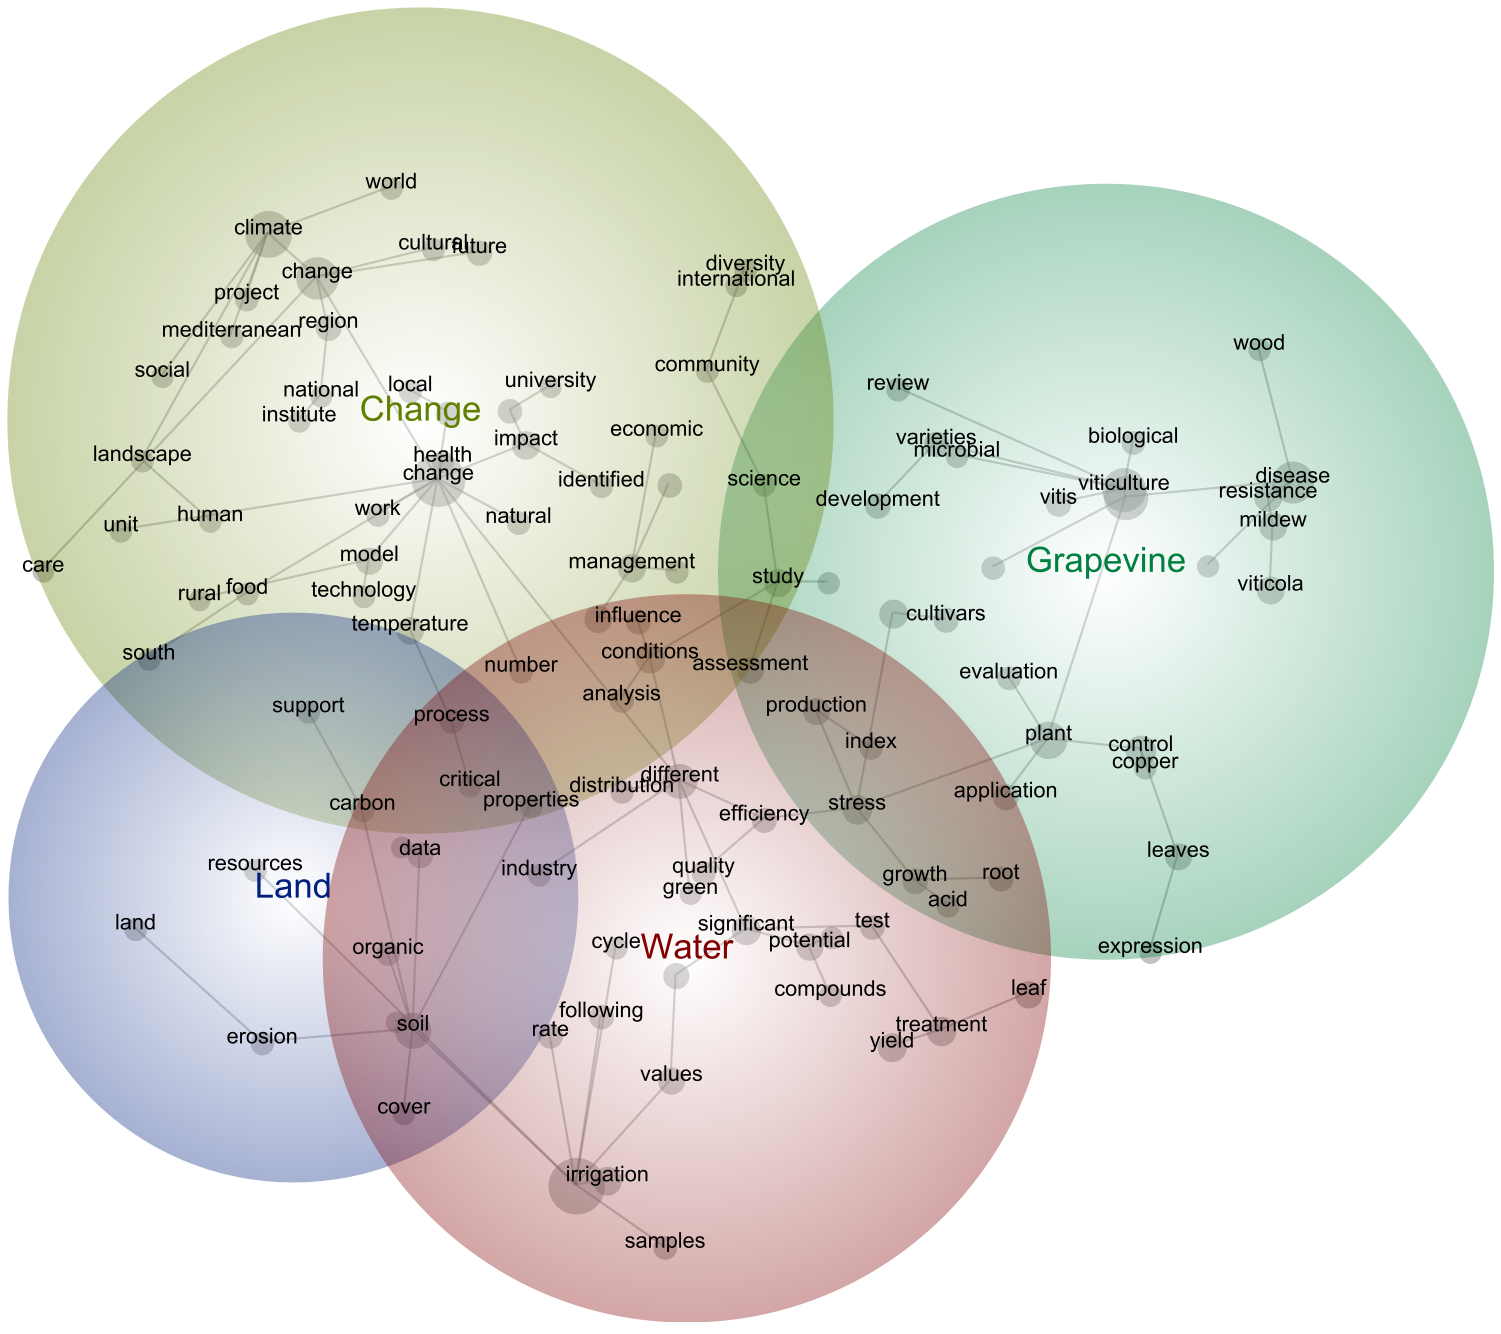
\includegraphics[width=\linewidth]{Winegrowing-concept-map}
    \caption{Your caption here}
    \label{fig:lexi}
\end{figure}

A key difference between the concepts from the literature search and the BN based on the industry panel was the rarity in how secondary and tertiary drivers of industry such as fuel or electricity use, were connected to primary sustainable concerns such as disease (even though disease was quite prominent in both). 
% With these concepts being related to the operations in fields as a result of changing practices or implementing different pest controls. Together these outputs provide a comprehensive overview of the key factors affecting environmental sustainability in the Australian winegrowing industry, offering valuable insights into areas of focus and potential improvement. This analysis underscores the multifaceted nature of sustainability, highlighting both the primary concerns and the interconnected secondary factors that must be managed on the ground.

\subsection{Region-specific BN: Coonawarra}

Identified key factors impacting environmental sustainability were examined with regard to Coonawarra. By comparing the generic Bayesian Network (Figure \ref{fig:b}) model to the Coonawarra-specific model (Figure \ref{fig:robyn} and Figure \ref{fig:marcel}), we identified regional characteristics that influence these variations. In this case study, we altered the general Australian BN to model and analyse the complex interactions between various environmental factors affecting wine production in Coonawarra. By incorporating industry-specific data and expert knowledge, the BN framework allowed us to quantify the impacts of key variables such as water use, agrochemical application, soil health, and climate conditions to each other. This approach not only aids in understanding the current sustainability status of the region but also helps in identifying potential areas for improvement and implementing effective management strategies. The resultant two models represent the final consensus, reflecting the diverse perspectives and occasionally differing viewpoints among the experts, necessitating the development of two distinct but complementary models.

    %     Sustainability in Coonawarra Winegrowing: Key Factors and Influences
    % #TODO: what are the regional specifics of coonawarra
    % How do the identified key factors vary across different wine regions in Australia, and what regional characteristics influence these variations?
    %     Purpose: Examine regional differences and tailor sustainability strategies.
    %     Results: Compare the generic model to the Coonawarra model. Acknowledge there is more work to be done here due to the amount of regions across Australia and the world. Prevous work also helps to illustrate these differences.

    % How do changes in key factors under various environmental and regulatory scenarios influence the overall environmental impact in Coonawarra?
    %     Purpose: Assess different factors overall influence to environmental sustainability given the definitions used.
    %     Results: Use the CPT values to assess the significant contribution of different variables on the BN and how that effects environmental sustainability.

\begin{figure}[h!]
    \centering
    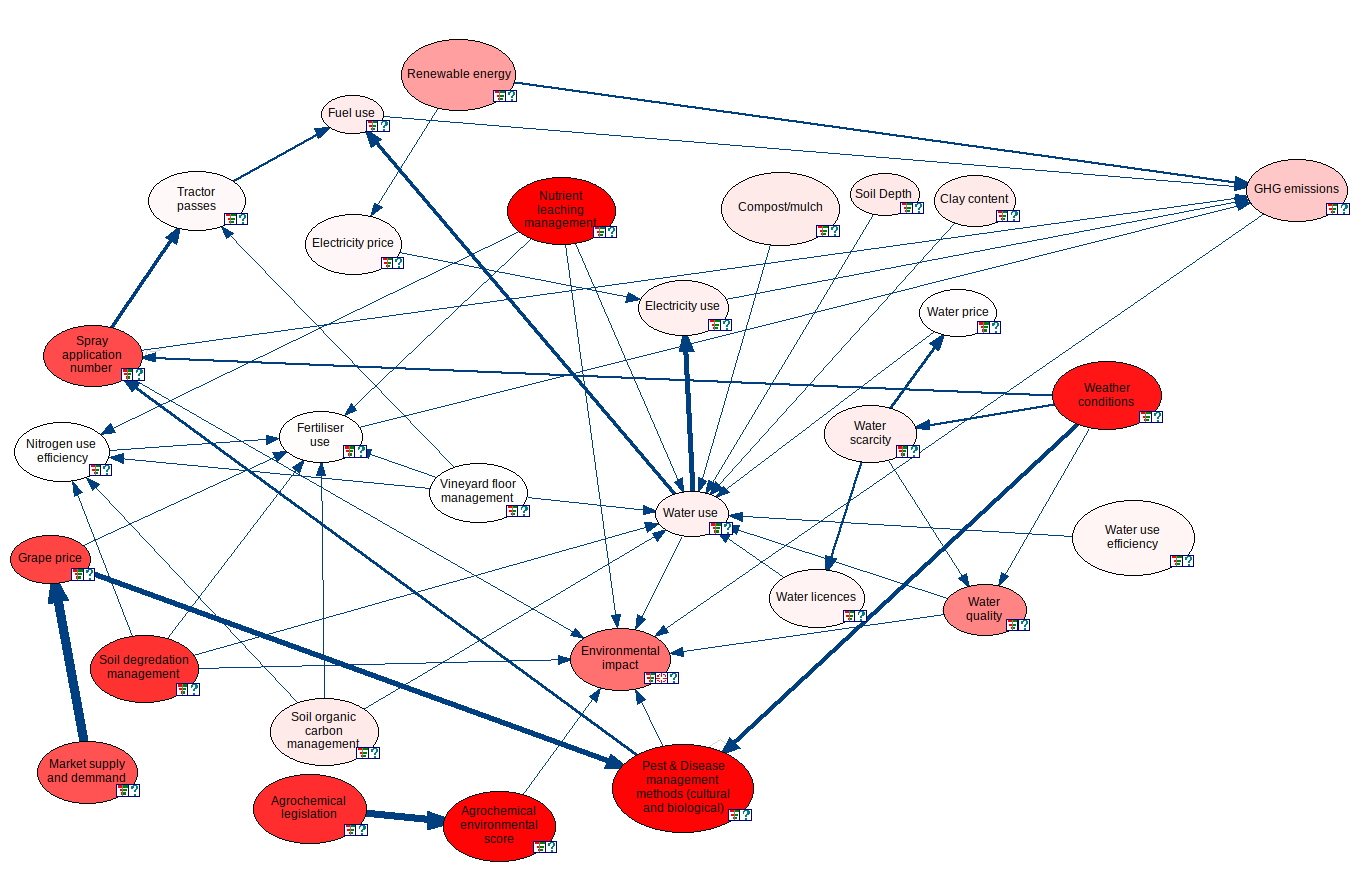
\includegraphics[width=\linewidth]{robyn}
    \caption{Coonawarra-specific Bayesian Network illustrating key factors impacting environmental sustainability, with nodes coloured by sensitivity to environmental impact.}\label{fig:robyn}
\end{figure}

\begin{figure}[h!]
    \centering
    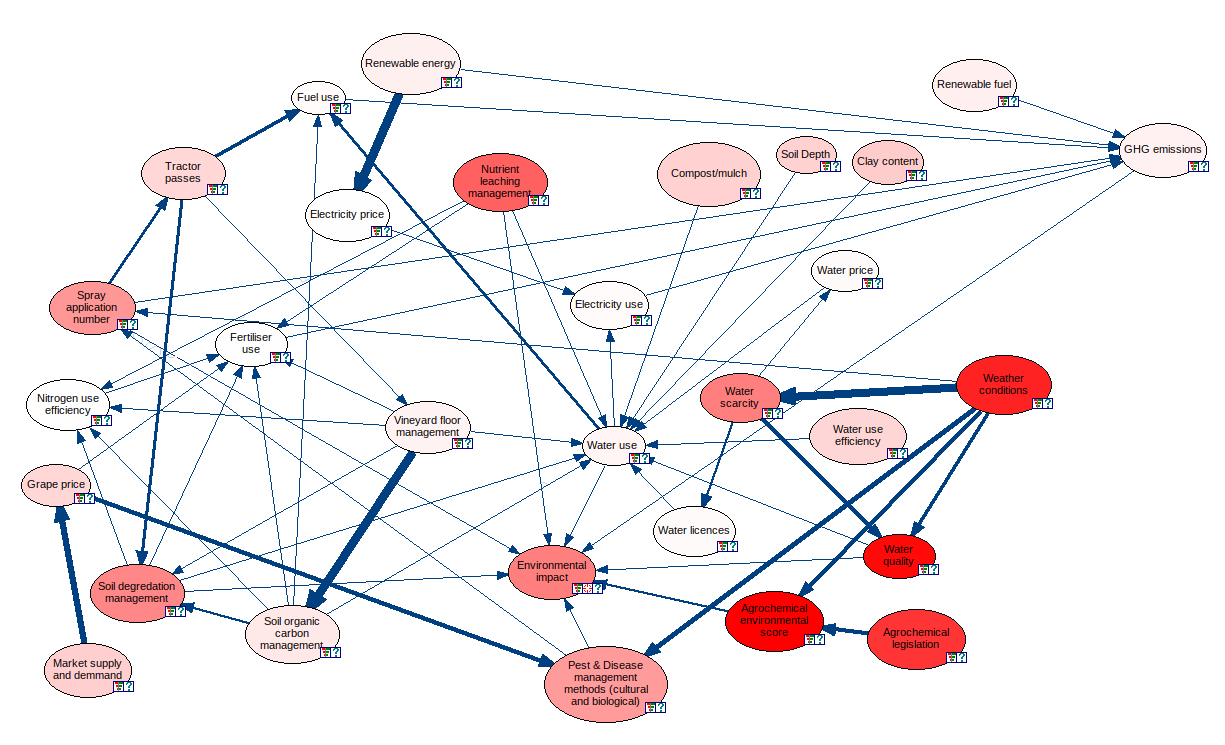
\includegraphics[width=\linewidth]{marcel}
    \caption{Coonawarra-specific Bayesian Network illustrating key factors impacting environmental sustainability, with nodes coloured by sensitivity to environmental impact.}\label{fig:marcel}
\end{figure}

% TODO: the exclusion of renewable fuels due to none being used in coonawarra
% the difference in vineyard floor management and its relationship to tractors
% The influence of compost, soil depth and clay content. although not specifically significant due to not listing the CPTs - it was highlighted as significant with different influence values depending on the direct field in question and not just which vineyard.
% variation occurs all the way to the vine level!

The comparison reveals that while some factors, such as water use and agrochemical legislation, remain consistently significant, other factors such as soil show variation not only at a regional level but sometimes at the paddock level as described by the expert panel. Figure \ref{fig:robyn} and \ref{fig:marcel} highlight the unique environmental and regulatory conditions specific to this region, indicating a need for tailored sustainability strategies. It is important to acknowledge that this analysis also illustrates that further work would be required to describe other regions or specific vineyards. 

The primary difference in interactions between the two BNs (see Figure~\ref{fig:robyn} and~\ref{fig:marcel}) lies in vineyard floor management and tractor passes. In one, greater tractor passes were used purposefully to manage the vineyard floor; the other managed vineyard floor as a consequence of tractor passes, leveraging opportunities when the tractor was used. This distinction highlights how operational decisions can vary based on regional practices and priorities. A point was also raised that scale can cause a further driving factor, where tractor passes may be greatly increased as an expense on larger plots of land. However, this issue as well as directly attributing measurable cause to granular specifics such as composting, soil depth and clay content cannot be fully addressed without site or paddock specific knowledge.

As a factor, water emerged as the most interconnected variable for both BNs, with edges connecting it to almost everything either directly or indirectly, illustrating its fundamental role in agriculture. The edges between different factors reveals that water is the most connected. Weather conditions also play a significant role, influencing water availability, quality and disease/pest pressures.Within both of the models, the most significant factors impacting environmental sustainability are water quality, pest and disease management, market pressures, agrochemical use, and climate/weather conditions. These factors were identified as having the highest sensitivity to environmental impact, indicating their crucial roles in the sustainability of the region.

The influence of factors on each other are described through the CPT values (see appendix) and allow for an in-depth analysis of how changes in key factors, under various environmental and regulatory scenarios, influence the overall environmental impact. For instance, the significant sensitivity that environmental impact had with regard to pests/disease, climate and agrochemicals compared to factors such as green house gas emissions. Importantly that these sensitive factors also link greatly to one another, highlighting how critical areas for regulatory and environmental interventions can be to multiple factors beyond their specific target. Furthermore, the relationships help to illustrate the further complexity of how these significant factors relate to these further considerations such as greenhouse gas emissions and the extended connection to fuel or electricity use. Where addressing issues such as disease can require the increased use of tractors and thus fuel.

The Coonawarra-specific BN supports the findings from the literature, with a more structured map of how factors interact compared to the automatically generated figures from tools like Leximancer. The BN provides a detailed view of the relationships between factors, highlighting the central role of water and the interconnectedness of pest management, market pressures, and climate conditions. Additionally, the BNs emphasise economic factors, such as market pressures and grape prices, and includes how they interact within a scope of secondary factors like fuel and electricity use.

% The other case study BN aligns with the literature by visually representing connections and highlighting significant factors through bibliometric analysis. However, the BN derived from the industry panel offers explicit connections and sensitivity analyses based on expert knowledge, providing a more nuanced understanding of the factors and their impacts compared to the broader mind maps generated from literature reviews.

The two case study BNs are almost identical in their significant factors and interactions. Both emphasize the importance of water quality, pest and disease management, and climate conditions. The primary difference is the sensitivity to tractor passes, water quality, water scarcity, and soil degradation management, with one model showing higher sensitivity to these factors. Aside from the role of tractor passes, there are no major differences between the two BNs. The similarity in significant factors and their interactions underscores the robustness of the BN approach in capturing the critical elements of environmental sustainability in winegrowing.

The findings from the case study align closely with the literature, illustrating more directly how factors that contribute to environmental sustaianbility are connected. The BNs provide a detailed and structured view of primary factors and their relationships to secondary and tertiary concerns within the industry. This detailed evaluation helps prioritise actions and policies that could lead to significant improvements in the sustainability practices of winegrowing regions.

% \subsection{Results notes}

% % =================================
% Structuring the Results Section Based on These Questions:
% Introduction to Results

%     Content: Briefly restate the refined research questions.
%     Explanation: Explain the approach to answering these questions using the BN model and CPT values.

% Primary Factors Identification

% Question: What are the primary factors that significantly impact environmental sustainability in the Australian winegrowing industry?

%     Content: Present the primary factors identified through your analysis.
%     Data: Use the rigorous definitions and the generic BN to highlight these factors.
%     Figures/Tables: Include a table or figure showing the key factors and their relative importance.

% Quantitative Measurement and Analysis

% Question: How can these key factors be quantitatively measured and analyzed to assess their contributions to sustainability in the Australian winegrowing industry?

%     Content: Describe the methods used to measure and analyze the key factors.
%     Data: Show measurements and analytical results from the CPT values in the specific BN models.
%     Figures/Tables: Include charts or tables showing the measurements and analyses.

% Relationships Between Factors

% Question: What are the direct and indirect relationships between these key factors and environmental sustainability in the Australian winegrowing industry?

%     Content: Discuss the direct and indirect relationships identified.
%     Data: Present interaction diagrams or tables.
%     Figures/Tables: Include a BN tree diagram illustrating these relationships.

% Regional Variations

% Question: How do the identified key factors vary across different wine regions in Australia, and what regional characteristics influence these variations?

%     Content: Compare the key factors and their impacts across different regions.
%     Data: Present comparisons between the two specific BN models from different growers.
%     Figures/Tables: Include figures comparing regional differences.

% Scenario Analysis

% Question: How do changes in key factors under various environmental and regulatory scenarios influence the overall environmental impact in the Australian winegrowing industry?

%     Content: Analyze the impact of different scenarios on environmental sustainability.
%     Data: Use scenario-based BN queries to show changes in key factors and their impacts.
%     Figures/Tables: Include charts or tables summarizing the scenario analysis results.

% Example Framework for Presenting Results:
% Introduction to Results

% "The results of this study are structured to address five primary research questions aimed at understanding the key factors and their interactions affecting the environmental impact of vineyards in the Australian winegrowing industry. The analysis leverages Bayesian Network models to provide a comprehensive view of these factors and their contributions."
% Primary Factors Identification

% Question: What are the primary factors that significantly impact environmental sustainability in the Australian winegrowing industry?
% Results:

%     Identified Factors: Water usage, pesticide application, soil management, etc.
%     Data Source: Defined terms provided by industry experts and the generic BN model.
%     Figures: Table 1 shows the key factors and their relative importance derived from the BN analysis.

% Quantitative Measurement and Analysis

% Question: How can these key factors be quantitatively measured and analyzed to assess their contributions to sustainability in the Australian winegrowing industry?
% Results:

%     Measurements: Quantitative analysis of key factors using CPT values from two specific BN models.
%     Data Source: CPT values from BN models of two growers.
%     Figures: Table 2 presents the measurements and analysis results.

% Relationships Between Factors

% Question: What are the direct and indirect relationships between these key factors and environmental sustainability in the Australian winegrowing industry?
% Results:

%     Interactions: Direct and indirect relationships as illustrated by the BN model.
%     Data Source: Generic BN model and specific models.
%     Figures: Figure 1 illustrates the BN tree diagram showing these relationships.

% Regional Variations

% Question: How do the identified key factors vary across different wine regions in Australia, and what regional characteristics influence these variations?
% Results:

%     Regional Variability: Comparison of factors and impacts across regions using specific BN models.
%     Data Source: BN models from two growers in different regions.
%     Figures: Figure 2 compares the BN models for different regions.

% Scenario Analysis

% Question: How do changes in key factors under various environmental and regulatory scenarios influence the overall environmental impact in the Australian winegrowing industry?
% Results:

%     Scenarios: Impact analysis under different scenarios using BN models.
%     Data Source: Scenario-based BN queries.
%     Figures: Table 3 summarizes the scenario analysis results.

% This refined approach ensures that your Results section directly addresses your research questions and clearly presents your findings. Let me know if there are specific details or sections you’d like further refined!

\section{Discussion}

This investigation highlights the key factors of Australian winegrowing that contribute to  environmental sustainability through the lens of BNs created with assistance from industry input. These models have established the intricate, and interconnected nature of various influences on environmental sustainability in Australian winegrowing. A keener understanding of how these factors both interact and effect one another from the perspective of research and industry is illustrated within these models, with a major outcome being the highlighting of water use's critical importance as one of the most interconnected variables. The influence of water use reached almost every variable, with its connection to operational decisions being reflected within its propagation to other factors such as tractor use, disease and pest prevention, as well as management strategies for soil. This finding aligns with water being the lifeblood of agriculture~\cite{chawlaWaterProductivityAgriculture2023}, essential for both the health of the vines and the broader ecosystem, especially within Australia's dry climate~\cite{australianbureauofstatisticsWaterUseAustralian2021}.

Of further significance was the management of pests and diseases, market pressures and climate. With these external influences being prominently connected to vineyard operations through their connection to factors such as fuel, tractor, water and electricity use. In particular, climate acted as an interface between water and pest/disease, due to climate being a determining factor in temperature and water availability which are highly influential to pests and disease~\cite{boisClimateVsGrapevine2017}. Of great concern to climate was how it influenced water availability, pest/disease pressures, and its overall contribution to vineyard health. Understanding these interactions is vital for developing adaptive management strategies that can cope with climate variability and change~\cite{agostaRegionalClimateVariability2012,alsafadiFutureScenariosBioclimatic2023,barriguinhaVineyardYieldEstimation2021,sharmaChapterImpactClimate2014}. In a more general sense climate and weather conditions are shown within the literature to be significant determinants of a variety of factors within vineyards such as yield~\cite{barriguinhaVineyardYieldEstimation2021,antonComparativeStudyRisk2012}, erosion~\cite{biddoccuEvaluationSoilErosion2020,doi:10.1177/0309133319861833}, and are further determinants of chosen grape varieties~\cite{topferGrapeVarietiesAre2022, petriashviliImpactClimateChange2023}. The BN models captured the complexity of how climate can propagate to these considerations through other factors; as well as how these other factors are connected.

The case study highlighted the direct influences on environmental sustainability, where environmental sustainability was found to be most sensitive to factors such as pests/disease, water use, economic pressures and climate which were found to be highly related through their connection to elements used in operational responses such as the use of agrochemicals and tractors (see Figures~\ref{fig:robyn} and~\ref{fig:marcel}). A major concern from the industry panel within these relationships was that, while necessary for maintaining vine health and productivity, excessive or inappropriate agrochemical use can lead to major negative environmental impacts~\cite{alonsogonzalezUnveilingTerroirEvaluating2024,manjarres-lopezAssessmentPesticideResidues2021}. The model emphasised the need for balanced and regulated agrochemical practices; and especially for such practices being followed appropriately~\cite{baianoOverviewSustainabilityWine2021}.

The findings from this study are consistent with the existing literature on sustainability in viticulture, which also identifies water management, pest/disease control, economic pressures, and climate conditions as key factors. Many of these singular relationships are well-defined within literature studies such as those between climate and pest/disease \cite{olatinwoChapterWeatherbasedPest2014}. Furthermore, literature  highlights a growing need for data and more decision support tools to assist with combatting external pressures such climate, water scarciy and disease \cite{naigeonDATADecisionmakingViticulture2023,stefaniniBayesianCausalModel2022,fincoCombiningPrecisionViticulture2022a,laurentLocalInfluenceClimate2022}. Tools such as Bayesian networks are becoming more applied to assist with the creation of decision support tools such as with water management \cite{carmonaUseParticipatoryObjectOriented2011} or vineyard placement \cite{abbalDecisionSupportSystem2016}. However, the combination of holistic approaches to reviewing sustainable practices in the adoption of techniques through measurable and holistic approaches is a growing need in policy creation and uptake of new novel sustainable practices \autocite{mayfieldDesigningExpertledBayesian2023,baianoOverviewSustainabilityWine2021,dichiaraCollaborativeApproachAchieving2024}. Although more holistic approaches are required to review the total accumulated benefits of sustainable practices, it is well aligned between researchers, the public and policy-makers that this endeavour is of great importance to the Australian agricultural industry as a whole \cite{dumbrellComparingAustralianPublic2024}.

The BN models provide structure to the broader way of how the major factors within literature interact, offering a clearer understanding of their interdependencies and relative sensitivity with regard to environmental sustainability as an outcome. The existing literature provides exceptional detailed understanding of many mechanisms behind the relationships explored within this study. The BN allows the further exploration of the peripheral connections beyond these relationships to be further considered. A strength behind the use of Bayesian Network is the ability to replace edges between nodes with any analysis that allows for the derivation of a posterior from some input prior; allowing for the BN to be used as a framework that can further integrate other studies results into these relationships~\cite{kimphuctranMachineLearningProbabilistic2022,kollerObjectOrientedBayesianNetworks1997,korbBayesianArtificialIntelligence2011}.

By linking fuel and electricity use with well-studied factors like water and climate, the BN model broadens the scope of sustainability research in viticulture, emphasising the interconnected nature of these challenges. Integrating elements which play critical roles in vineyard operational decisions such as tractor, fuel and electricity use, which were more peripheral within the bibliometric analysis, to central themes like water, pests/disease and climate offered a holistic view of sustainability in winegrowing. The model demonstrated how fuel, tractor, and electricity use are intertwined with factors such as water and climate through propagation. Even though environmental sustainability was not highly sensitive to such factors, they directly relate to operational decisions that can be influenced by growers over a season. For example, electricity and fuel use are crucial for irrigation systems, as well as fuel use and tractors required for operations linked to soil preparation, management, and pest/disease control actions. Notably these operational decisions can be preventative or reactionary within a season. With many of these decisions being directly influenced by the central themes described in the bibliometric analysis (soil, water and disease) particularly all of which are connected to climate~\cite{fragaClimateChangeNew2020,tofaloClimateChangeWine2023,naigeonDATADecisionmakingViticulture2023}. Additionally, the need to adapt to changing climate conditions can drive increased use of fuel and electricity, potentially exacerbating greenhouse gas emissions. The findings align with literature, with researchers highlighting how different operations contribute to climate change through greenhouse gas emmissions \cite{pilafidisAssessingEnergyUse2023,cechPesticideUseAssociated2022,zhangEstimatingEconomicEnvironmental2019} and conversely how climate change increases pressure on farmers~\cite{barnaEditorialImprovingSustainability2023,costaRoleSoilTemperature2023,atakClimateChangeAdaptive2024}, suggesting future research should focus on integrated resource management, technological innovations to reduce energy consumption, and policy incentives to promote energy-efficient practice~\cite{pereiraViticultureClimateChange2023}. This integrated perspective is crucial for developing effective strategies to enhance the sustainability of the winegrowing industry.

The integration of expert knowledge was an essential part of constructing these BNs, particularly in defining the structure of the network and the CPTs. However, even within this analysis, disagreements were present amongst the panel especially as the models became more granular. The model is limited by the knowledge of the expert panel and by its specificity to the Australian, and further the Coonawarra context. The model created is also limited, in that, it solely represents the outcomes of a single season in isolation. No further accounting for past or future factors that may affect vineyard outcomes or decisions were considered. A dynamic Bayesian network could potentially address this issue but would require further investigations regarding the temporal factors that occur between seasons. Although this is a limiting factor, the model created within this study could still operate as the central static consideration between these temporal factors if future research was conducted. Similarly, spatial influences are also difficult to generalise to. Factors influencing sustainability in one winegrowing region may differ significantly from those in another region due to variations in climate, soil types, management practices, and economic conditions. Therefore, the applicability of the BN developed for the Coonawarra region does not extend seamlessly to other wine regions. The more general model for Australia would also need to be altered to generalise to other countries due to the wide and varying circumstances that exist from country to country.

The BN models helped to illustrate how economic incentives can be drivers of sustainable practices. The definitive influence and relationships between what are more tertiary considerations of environmental sustainability being directly connected to further considerations such as operational costs. Market pressures, including the demand for high-quality grapes through factors such as grape prices, were found to have an impact on sustainability practices but were limited in this study through only reviewing them within the lens of environmental sustainability. The ability to effectively gauge whether operations could afford to engage further with management programs for factors such as soil, pests, disease etc was in part driven by the economic climate provided to growers as well as what may be much more specific circumstance; of which is a potential further avenue of research that would compliment this work significantly.

\section{Conclusion}

This study provides an in-depth examination of environmental sustainability in Australia and the Coonawarra winegrowing region using BNs. Through integrating industry expertise and empirical data, the BN models developed in this research offered a structured and quantitative framework for understanding the complex interactions amongst key factors influencing environmental sustainability. The findings highlight the critical role of water quality and availability, emphasising its critical influence on all operational decisions either directly or propagating through other factors. With this critical nature being due to water being the most interconnected factor. With this high interrelatedness emphasising the importance efficient water management practices enhancing sustainability in viticulture.

Pest and disease management emerged as another significant factor, with effective control strategies having the potential to mitigate excessive agrochemical use and its associated environmental impacts. The study also identified the substantial impact of market pressures and economic factors on sustainability practices, illustrating how economic incentives can drive or hinder sustainable vineyard management. Of significant relation both in the literature and the BN was climate's influence on all of these factors as well as overall vineyard health. The BN models captured the intricate ways these factors interact, highlighting the need for adaptive management strategies to cope with climate variability and change. With these factors all being connected in someway within the model through propagation across the BN.

The comparative analysis with existing literature affirmed the relationships explored by the expert panel adding robustness of the study's findings. With the BN itself, aligning well with previously identified key factors while providing a more detailed map of their interdependencies. The BN approach not only confirmed known relationships but also illustrated how these relationships looked holistically across sustainability within the winegrowing industry.

Overall a comprehensive analysis of key factors and their interactions within the Australian winegrowing industry was gained. The use of BN models for further regions could help to inform more specific targeted interventions and policy-making, aiding in the promoting of sustainable practices in the winegrowing industry. The integration of expert knowledge and empirical data in this research demonstrates the potential of BNs as powerful decision support tools for sustainability analysis and decision-making in agriculture. With the potential to enhance this research being the further incorporation of time, other regional specific considerations and economic outcomes related to these environmental concerns.

\section{References}
% Your references text goes here.
\bibliographystyle{plain}
\bibliography{references}

\end{document}
